\documentclass[8pt]{beamer}
\usetheme{default} % Very simple theme
\usecolortheme{dove} % Minimalist grayscale colors
\setbeamertemplate{navigation symbols}{} % Remove navigation bar

\usepackage{graphicx} % Package for images
\graphicspath{{figs/}} % Path to your figures directory
\usepackage{array}  % For better column spacing
\usepackage{caption} % Required for \captionof

% Title Information
\title{Stochastic methods in water resources}
\subtitle{Lecture 1: Course introduction, definition of stochastic hydrology, other definitions}
\author{Luis Alejandro Morales, Ph.D.}
\institute{Universidad Nacional de Colombia} %// Department of Civil and Agriculture Engineering}
\date{\today}

\begin{document}

% Title Slide
\begin{frame}
    \titlepage
\end{frame}

%--------
\section{Some definitions in hydrology}
\begin{frame}{Some definitions}
    \begin{block}{Hydrological sciences}
        Hydrology is an earth science concerned with the dynamics in space and time of water across different compartments (\textbf{water cycle}). Hydrology studies the source and fate of water in liquid, gaseous, and solid states on earth. It also studies water quality. 
    \end{block}    
    \centering
    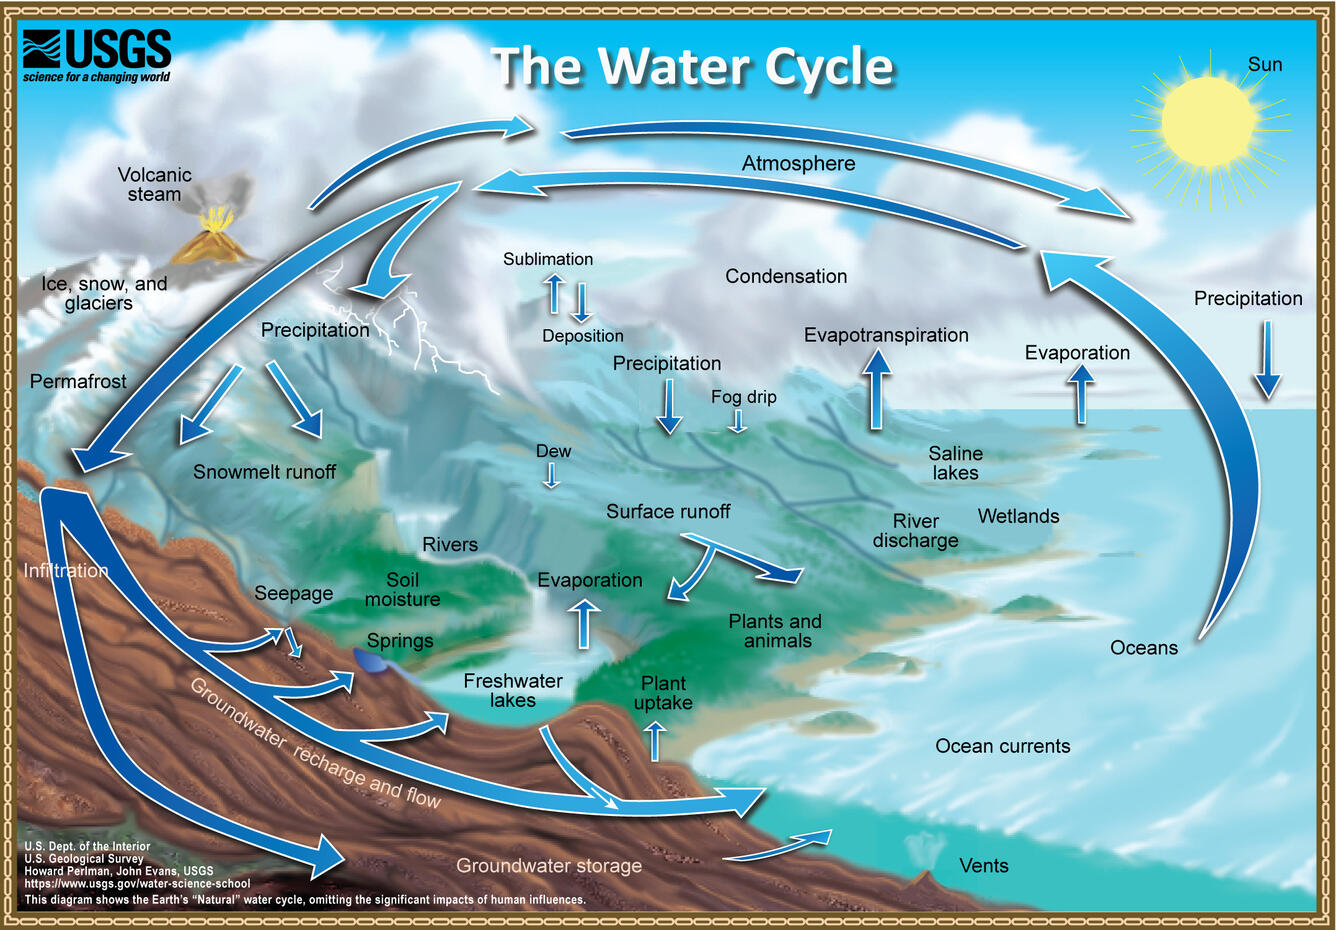
\includegraphics[height=0.7\textheight, keepaspectratio]{water-cycle-natural.jpg}
\end{frame}

\begin{frame}{Some definitions}
    \begin{block}{Hydrological environments}
        Hydrological environments is where hydrological processes occur and are part of the \alert{water cycle}. Here are the relationships of hydrological environments and processes:
        \begin{tabular}{p{4cm}p{0.5cm}p{6cm}}  % No vertical bars
                \hline
            \alert{Environment} & & \alert{Process}  \\
                \hline
    Oceans and seas &  $\rightarrow$ & Evaporation and storage \\
    Atmosphere & $\rightarrow$ & Evapotranspiration storage \\
    Continental solid (e.g. glaciers) and liquid (e.g. river and lakes) waters & $\rightarrow$ & Storage \\
    Land surface soils and plants & $\rightarrow$ & Infiltration, canopy interception,  evapotranspiration, water retention, snow and ice accumulation, melting, interflow, overland flow and base flow \\
    Earth's crust surface layer & $\rightarrow$ & Storage
\end{tabular}
        Water quality is also affected within the hydrological environments. Water and energy fluxes are interchanged among environments:
        \begin{itemize}
            \item Oceans and seas $\rightleftharpoons$ atmosphere
            \item Land surface soils and plants $\rightleftharpoons$ Atmosphere
            \item Land surface soils and plants $\rightleftharpoons$ Continental waters 
        \end{itemize}
        Any hydrological environment \alert{receives}, \alert{releases} and/or \alert{storage} flow.  This is why the sequence of \alert{input} $\rightarrow$ \alert{storage} $\rightarrow$ \alert{output} constitute the  basic components of a \alert{hydrological system} that represents a \alert{hydrological process} in space and time. Hydrological processes in nature are \alert{stochastic} or \alert{deterministic} or a mix of both. A pure deterministic process es one that occurs under controlled artificial conditions.
    \end{block}    
\end{frame}

\begin{frame}{Some definitions}
    \begin{block}{Model definition according to system's theory}
        A model is a simplified representation of a prototype (reality), and they can be physical or mathematical models. Mathematical models are composed by:
        \begin{itemize}
            \item \alert{Boundary conditions}: Physical boundaries of the prototype that define how the system interact with the exterior. 
            \item \alert{State variables}: Describe and  define the model at a certain time and space. These variables change in space and time.  
            \item \alert{Input variables}: Variables originated outside model's boundaries and are observed data. This includes initial condition (when $t=t_0$).
            \item \alert{Parameters}: Parameters are usually model constant that change spatially only. Serve to represent model processes or properties.  
            \item \alert{Output variables}: Or response variables are originated from the input and the state variables throught the parameters. They change in space and time. 
            \item \alert{Constant}: Constants are properties that do not change in space and time. E.g. fluid properties and gravity. 
        \end{itemize}
    \end{block}    
\end{frame}

\begin{frame}{Model definition according to system's theory}
    \begin{minipage}{0.495\textwidth}
    From the continuity equation:
\vspace{-5pt}
$$
    \frac{ds}{dt} = I - O
\vspace{-5pt}
$$
    where $s$ is the sytem's storage as a function of time ($t$),  and $I$ and $O$ are inputs and outputs of the system, respectively. From the figure, this equation is expressed as:
\vspace{-5pt}
    $$
    \frac{ds}{dt} = \left( p(t) - et(t) - i(t)\right)A - q(t)
\vspace{-5pt}
    $$
    where $p(t)$ is the precipitation in $L T^{-1}$, $et(t)$ is the evapotranspiration  in $L T^{-1}$, $i(t)$ is the infiltration in $L T^{-1}$, $q(t)$ is the outflow in $L^{3} T^{-1}$ and $A$ is the catchment's area in $L^{2}$. Also in the figure, $k$ is an storage coefficient in $T^{-1}$ and $r$ is the infiltration capacity in $L T^{-1}$.
    Note that $s(t)$ is the \alert{state variable}; $p(t)$ is the \alert{input variable}; $q(t)$, $et(t)$ and $i(t)$ are  \alert{output variables}; $k$ and $r$ are \alert{parameters}; and $A$ is a \alert{constant}. From the equation above:
\vspace{-5pt}
$$
s^t = s^{t-1} + \left[ \left( p^{t} - et^{t}  - i^{t} \right) A - q(t) \right] \Delta t
\vspace{-5pt}
$$
where $i(t)= r$ and $q(t)=s(t) k$. So:
\vspace{-5pt}
$$
s^t = s^{t-1}\left(1-k\Delta t \right) + \left[ \left( p^{t} - et^{t}  - r \right) A \right] \Delta t
\vspace{-5pt}
$$
\end{minipage}
\hfill
\begin{minipage}{0.495\textwidth}
    \centering
    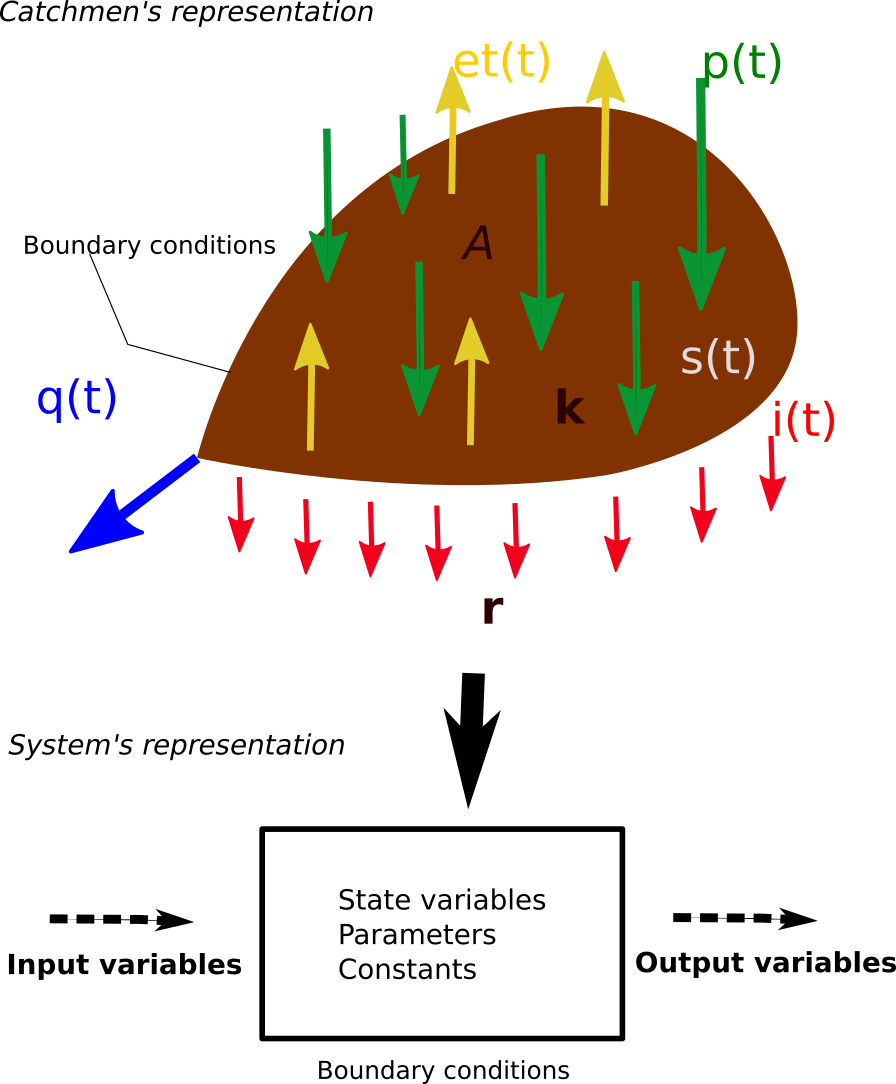
\includegraphics[height=0.8\textheight, keepaspectratio]{fi2l1.png}
    %\captionof{figure}{Annual maximum discharges of the Danube River at Orshova Romania. 1) time series of maximum, 2) time series mean and 3) time series trend.}
\end{minipage}
\end{frame}



\section{Why stochastic methods in hydrology?}
\begin{frame}{Why stochastic methods in water resources?}

    \begin{block}{Stochastic methods}
    According to \cite{}, "stochastic methods thus aim at predicting the value of some variable at non-observed times or at non-observed locations, while also stating how uncertain we are when making these predictions".
    \begin{figure}
    \centering
    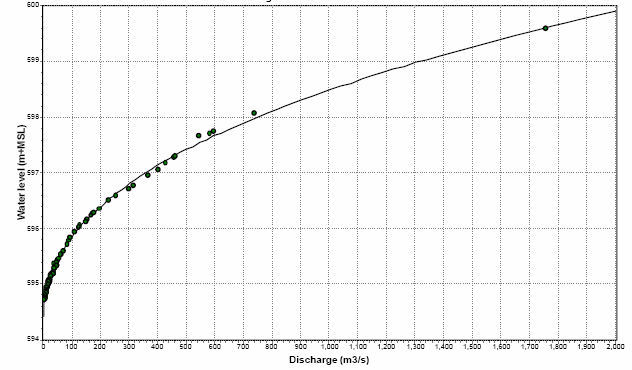
\includegraphics[width=0.9\textwidth]{fi1l1.png}
    \end{figure}
    \alert{Uncertainty} is the key factor for the implementation of stochastic methods.  For instance, when observed ($Q$) and estimated ($\hat{Q}$) discharges are compared, there are some diferences (\alert{residuals}) between the two data sets ($e = \hat{x}-x$). 
\end{block}
\end{frame}

\begin{frame}{Why stochastic methods in water resources?}
    Errors  can be summarized as:
    \begin{itemize} 
        \small
        \item \alert{Observation error}: Errors are always present in observations. Also external factor such air temperature and pressure can influence on water level records.
        \item \alert{Errors in boundary conditions}: In watershed hydrological modelling, the definition of boundary conditions,  most of the time,  does not account for flow exchange between neigbour basins, particularly, groundwater flow exchange bringing in uncertainty in water balance estimates. 
        \item \alert{Errors in initial conditions}: Usually, initial conditions (initial values of state variables) are unknown at the beginning of model simulations causing uncertainty in model estimates. To correct it, models are "warm up" to pre-estimate initial conditions in order to reduce uncertainty.
        \item \alert{Errors in input data}: Such errors are very common in watershed modelling. Input data to rainfall-runoff models such as precipitation or evaporation are difficult to observed for large areas so large errors are possed on data causing uncertainty in model's estimates.  
        \item \alert{Errors due to unknown heterogeneity and parameters}: Unknown heterogeniety in processes representation is common in computational modelling as physical processes are oversimplified in models. Such simplifications, of course, do not capture process's heterogeneity inducing to errors. Vegetation properties and soil hydraulic conductivity are very heterogenous in space and time and difficul to represent correctly. Parameters that represent physical processes or properties are higly variable in space and time, however, modelling assume unique parameters for large areas and time frames leading to errors in model estimates. 
        \item \alert{Errors due to scale discrepancies}: Model's domains usually assume homegenety at certain scale. For instance, in a distributed hydrological models if the size of a cell in the computational grid is 1km x 1km, it is assume that processes representation does nos change is continuous and homegeneous in the cell. This ignore the changes in the cell leading ot uncertain estimates. 
        \item \alert{Model errors}: \emph{all models are wrong, but some are useful} by George Box. Models are an approximate representation of reality because they do not include all the intricate mechanism and interations that occur in natural systems. For instance, when surface flow is modelled the approximation of kinewatic wave is not always according to reality since small gradients of water level dominate the flow. 
    \end{itemize} 
\end{frame}

\section{Deterministic hydrology vs Stochastic hydrology}
\begin{frame}{Deterministic hydrology vs Stochastic hydrology}
    
    \begin{tabular}{p{5.5cm}p{5.5cm}}  % No vertical bars
    \hline
    \alert{Deterministic hydrology} & \alert{Stochastic hydrology} \\
    \hline
    Result from physical, chemical and biological deterministic laws, particularly from fluid mechanics and thermodynamics laws & Most of physical processes in nature are governed by laws of chance (stochastic or random) \\ \hline
    State variables are related to each other to represent fundamental laws throuhg mathematical expressions & The response of physical processes are governed by laws of change where every variable is a stochastic variable. \\\hline
    \emph{E.g. The response (runoff) of a impervious surface to a specific rainfall event with negligible evaporation and infiltration processes.} & \emph{E.g. Runoff, precipitation, evaporation, sediment transport, etc} \\\hline
    \emph{E.g. A rating function on the form of $Q = f(y)$ where $Q$ represent discharge through a fix-bed river cross section and $y$ water level stage.} &  \emph{E.g. The the annual precipitation at a point or over an area or other hydrological process at annual scale where no deterministic components are presented.}\\ \hline
    \end{tabular}
    \begin{itemize}
        \item Note that \emph{stochastic} $\rightleftharpoons$ \emph{change} $\rightleftharpoons$ \emph{random} $\rightleftharpoons$ \emph{probabilistic} are interchangeable. 
        \item There are no pure deterministic processes in hydrology; contrary, these are a combination of conservation and change laws.  
        \item Hydrological processes can be a combination of both: e.g. periodic behaviour (deterministic trigonometric function) $+$ random variation  $\rightarrow$ \alert{periodic-stochastic process}
        \item Note that a deterministic relationship function between random variables is also a random variables. E.g. The response of a river basin (runoff) to rainfall events is better understood by analysing not only the deterministic relationships but also the stochastic properties of observed rainfall, runoff, climate and basin data. 
    \end{itemize}
\end{frame}

\begin{frame}{Deterministic hydrology vs Stochastic hydrology}
\begin{minipage}{0.49\textwidth}
    \centering
    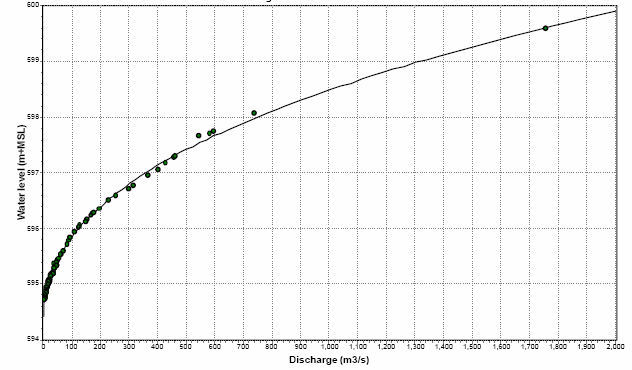
\includegraphics[width=\textwidth]{fi1l1.png}
    \captionof{figure}{Typical rating curve.}
\end{minipage}
\hfill
\begin{minipage}{0.49\textwidth}
    \centering
    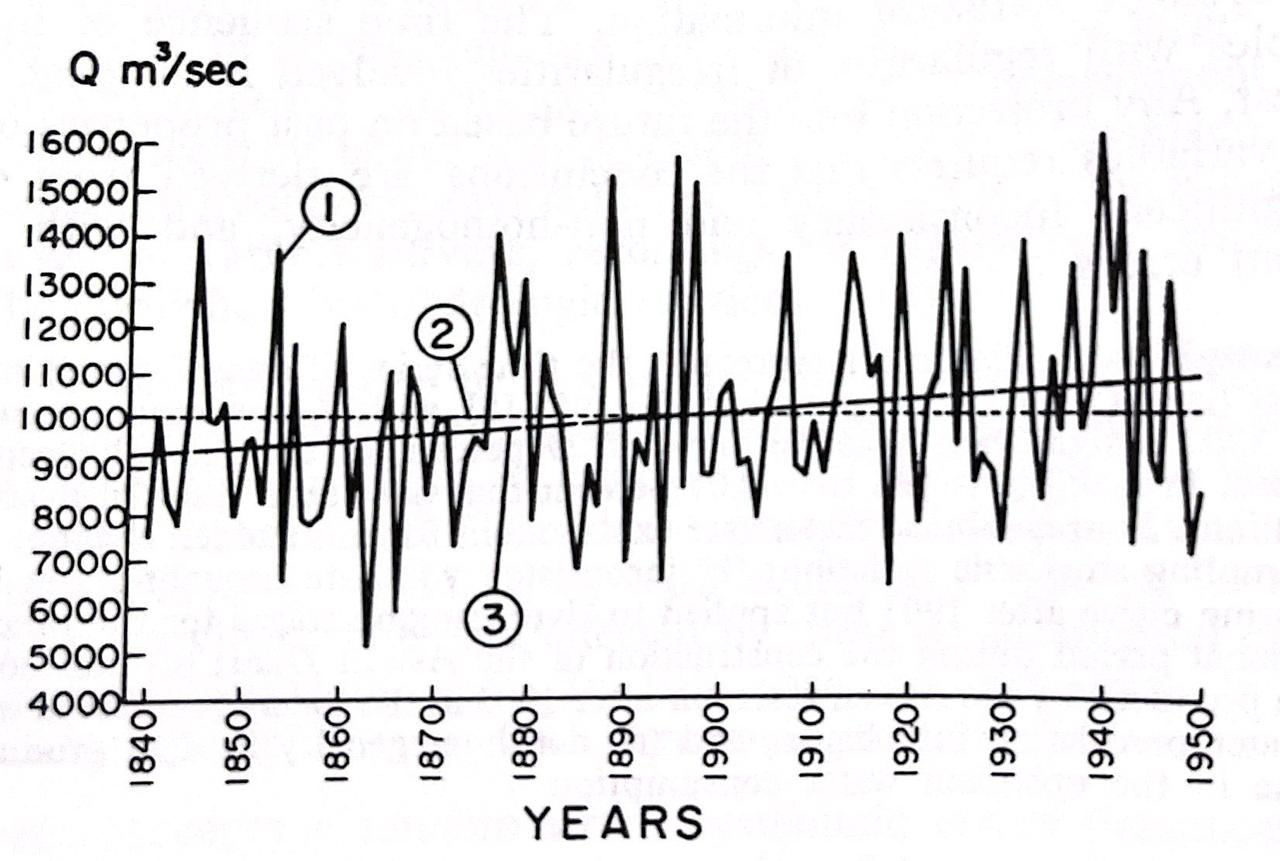
\includegraphics[width=\textwidth]{fiVu1_2.jpeg}
    \captionof{figure}{Annual maximum discharges of the Danube River at Orshova Romania. 1) time series of maximum, 2) time series mean and 3) time series trend.}
\end{minipage}
\end{frame}



\end{document}
